\documentclass[sigconf]{acmart}

\usepackage{mathptmx}
\usepackage{amsmath}
\usepackage{tikz}
\usepackage{pgfplots}
\usepgfplotslibrary{groupplots}
\usepgfplotslibrary{colorbrewer}
\usepackage{datatool}
\usepackage{ifthen}
% Curly braces
\usetikzlibrary{arrows.meta,decorations.pathreplacing,angles,quotes,patterns}
% Relative positioning
\usetikzlibrary[positioning]

\usepackage[binary-units]{siunitx}
\DeclareSIUnit\dBm{\dB\text{m}}

\tikzset{annotation/.style={scale=0.85,fill=white,inner sep=1,outer sep=3}}
\tikzset{txarrow/.style={-{Latex[scale=1.5]},dashed}}

\makeatletter
\def\pgfplots@stacked@diff{}
\makeatother

\definecolor{inkscape-royalblue}{RGB}{65,105,225}
\definecolor{inkscape-firebrick}{RGB}{178,34,34}
\definecolor{inkscape-forestgreen}{RGB}{85,155,85}
\definecolor{inkscape-khaki}{RGB}{240,230,140}
\definecolor{inkscape-lightsteelblue}{RGB}{176,196,222}

\definecolor{verylightgray}{gray}{0.85}
\definecolor{lightgray}{gray}{0.75}
\definecolor{darkgray}{gray}{0.5}

% x, y, color, prefix for node names, scaling
\newcommand{\tikzdrawframe}[5]{
	\node [draw,fill=white,rectangle,minimum height=4*#5,minimum width=3] (#4_preamble) at (#1,#2) {};
	\node [draw,fill=#3,rectangle,minimum height=10*#5,minimum width=3] (#4_payload) [below=of #4_preamble] {};
}

% x, y, node name
\newcommand{\tikzdrawwindow}[3]{
	\node [draw,dotted,fill=white,rectangle,minimum height=4,minimum width=10] (#3) at (#1,#2) {};
}

% from https://tex.stackexchange.com/a/178632
\pgfplotsset{
	discard if not/.style 2 args={
		x filter/.code={
			\edef\tempa{\thisrow{#1}}
			\edef\tempb{#2}
			\ifx\tempa\tempb
			\else
			\def\pgfmathresult{inf}
			\fi
		}
	}
}

\DeclareSymbolFont{symbolsb}{OMS}{cmsy}{m}{n}
\SetSymbolFont{symbolsb}{bold}{OMS}{cmsy}{b}{n}
\DeclareSymbolFontAlphabet{\mathcal}{symbolsb}


\begin{document}
\begin{minipage}{85mm}
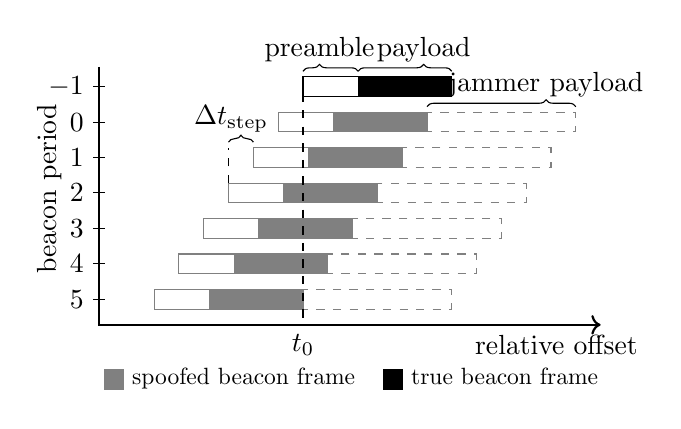
\begin{tikzpicture}
	% How many spoofed beacons should be drawn?
	\pgfmathsetmacro{\stepcount}{6}
	% Margin at the top of the picture
	\pgfmathsetmacro{\margintop}{0.3}
	% Height of a beacon bar
	\pgfmathsetmacro{\bcnheight}{0.25}
	% Gap between beacon bards
	\pgfmathsetmacro{\bcngap}{0.2}
	% Width of a symbol, main horizontal scaling factor
	\pgfmathsetmacro{\symbwidth}{0.07}
	% Margin on the left/right
	\pgfmathsetmacro{\ymargin}{10*\symbwidth}
	% All other properties are derived
	\pgfmathsetmacro{\lpreamble}{10*\symbwidth}
	\pgfmathsetmacro{\lpayload}{17*\symbwidth}
	\pgfmathsetmacro{\lbeacon}{\lpreamble+\lpayload}
	\pgfmathsetmacro{\ljammer}{\lbeacon}
	\pgfmathsetmacro{\stepsize}{\lbeacon/\stepcount}
	\pgfmathsetmacro{\xmin}{-\lbeacon-\ymargin}
	\pgfmathsetmacro{\totalheight}{\margintop+(\bcngap+\bcnheight)*(\stepcount+1)}
	
	% Axes
	\draw [->,thick] (\xmin,\totalheight-\margintop+\bcnheight/2) coordinate (yaxis)
	|- (\lbeacon+\ljammer,0) node (xaxis) [below,xshift=-16pt] {relative offset};
	\node at (\xmin,\totalheight/2) [rotate=90,yshift=18pt] {beacon period};
	
	% legitimate beacon
	\pgfmathsetmacro{\bcntop}{\totalheight-\margintop}
	\draw[color=black] (0,\bcntop) rectangle
		(\lpreamble,\bcntop-\bcnheight);
	\draw[decoration={brace,raise=2pt,aspect=0.3},decorate] 
		(0,\bcntop) -- node[above,pos=0.3,yshift=2pt] {preamble} (\lpreamble,\bcntop);
	\draw[fill=black,color=black] (\lpreamble,\bcntop) rectangle
		(\lbeacon,\bcntop-\bcnheight);
	\draw[decoration={brace,raise=2pt,aspect=0.7},decorate]
		(\lpreamble,\bcntop) -- node[above,pos=0.7,yshift=2pt] {payload} (\lbeacon,\bcntop);
	\draw ([xshift=2pt]\xmin,\bcntop-\bcnheight/2) --
		([xshift=-2pt]\xmin,\bcntop-\bcnheight/2) node[left] {$-1$};
	
	% spoofed beacons
%	\foreach \s in {0,...,\stepcount-1} {
	\foreach \s in {0,...,5} {
		\pgfmathsetmacro{\bcntop}{\totalheight-\margintop-(\s+1)*\bcnheight-(\s+1)*\bcngap}
		\pgfmathsetmacro{\bcnstart}{0-\stepsize*(\s+1)}
		\draw[color=darkgray] (\bcnstart,\bcntop) coordinate (bcnstart\s)
			rectangle (\bcnstart+\lpreamble,\bcntop-\bcnheight);
		\draw[fill=darkgray,color=darkgray] (\bcnstart+\lpreamble,\bcntop)
			rectangle (\bcnstart+\lbeacon,\bcntop-\bcnheight);
		\draw[dashed,color=darkgray] (\bcnstart+\lbeacon,\bcntop) coordinate (bcnend\s)
			rectangle (\bcnstart+\lbeacon+\ljammer,\bcntop-\bcnheight);
		\coordinate (bcnjamend\s) at (\bcnstart+\lbeacon+\ljammer,\bcntop);
		\draw ([xshift=2pt]\xmin,\bcntop-\bcnheight/2) --
			([xshift=-2pt]\xmin,\bcntop-\bcnheight/2) node[left] {$\s$};
	}

	% jamming label
	\draw[decoration={brace,raise=2pt,aspect=0.8},decorate] 
	(bcnend0) -- node[above,pos=0.8,yshift=2pt] {jammer payload} (bcnjamend0);

	% t step label
	\draw[dashed] (bcnstart2) -- (bcnstart2 |- bcnstart1);
	\draw[decoration={brace,raise=2pt,aspect=0.5},decorate]
	(bcnstart2 |- bcnstart1) -- node [above,pos=0.1,yshift=2pt] {$\Delta t_\text{step}$} (bcnstart1);

 % Vertical t_beacon line
	\draw[dashed] (0,\totalheight-\margintop) --
		(0,0) coordinate (t_beacon) node[below] {$t_0$};

	\node (truelbl) [below=-0.1 of xaxis,scale=0.85,xshift=-22pt] {{\strut}true beacon frame};
	\node (trueicon) [left=0 of truelbl,fill=black,draw=black,minimum height=.25cm,minimum width=.25cm,inner sep=0, outer sep=0] {};
	\node (atklbl) [left=0.25 of trueicon,scale=0.85] {{\strut}spoofed beacon frame};
	\node (atkicon) [left=0 of atklbl,fill=gray,draw=gray,minimum height=.25cm,minimum width=.25cm,inner sep=0, outer sep=0] {};
\end{tikzpicture}
\end{minipage}
\end{document}
